\documentclass[11pt,a4paper]{article}
\usepackage[T1]{fontenc}
\usepackage[margin=2.3cm]{geometry}
\usepackage{amsmath,amssymb}
\usepackage{graphicx}
\usepackage[dvipsnames]{xcolor}
\usepackage{enumitem}
\usepackage[colorlinks=true,linkcolor=blue,urlcolor=blue]{hyperref}
\setlength{\parskip}{0.6em}
\setlength{\parindent}{0pt}
\begin{document}

\begin{center}{\LARGE\bfseries openloan}\\[0.4em]{\large Compare loan EMIs and see how interest compounds, in three sessions.}\\[0.2em]\small PAN IIT OSS explainer \textbullet{} secondary school to diploma / undergraduate (levels 3-5)\end{center}

\section*{Why this exists}
Every loan quietly applies one rule: interest is charged on what you still owe. This explainer shows the mathematics behind that, from simple versus compound interest to the EMI formula, using only arithmetic and a short simulation. All lenders and rates are made up.

\section*{The end goal}
Compare loan EMIs and see how interest compounds. The end goal is to compare loan EMIs and see how interest compounds: given two offers, work out which is cheaper in total, what its true yearly rate is, and how prepayment changes it. This is general education, not financial advice.

\section*{How the three sessions build up}
\begin{enumerate}[nosep]
\item \textbf{Session 1: Why you pay back more than you borrowed} (Level 1, conceptual interactive model, 60 min).
\item \textbf{Session 2: Compound growth and the EMI} (Level 2, mathematical engineering model, 75 min).
\item \textbf{Session 3: Simulating real loans: prepayment, rate changes and flat rates} (Level 3, simulation and validation, 90 min).
\end{enumerate}

\section{Session 1: Why you pay back more than you borrowed}

\subsection*{A. Real-world problem}
A friend lends you 10000 units today and wants only 10000 back. A bank charges interest: you will pay back more than you borrowed. How much do you owe after 3 years if the interest is 10 percent a year? And why does a debt that adds interest to itself grow faster and faster? This repo is general education with made-up lenders and rates; it is not financial advice.

\subsection*{B. Concept and theory}
The principal P is the amount borrowed. The rate r is the yearly interest as a fraction (10 percent is 0.10). With simple interest the lender charges r P every year on the original P only, so after t years you owe A = P (1 + r t). With compound interest each year's interest is added to the debt, so the next year's interest is charged on a bigger amount: the debt is multiplied by (1 + r) every year and after t years you owe A = P (1 + r)\textasciicircum{}t. After one year the two are equal; after that compound interest is larger. Simple interest grows along a straight line, compound interest along a curve that bends upwards.

\begin{itemize}[nosep]
\item P: principal: the amount borrowed (units (any currency))
\item r: interest rate per year as a fraction (0.10 = 10 percent) (per year)
\item t: time (years)
\item A: amount owed after t years (units)
\end{itemize}

\begin{equation*}
A_{\text{simple}}=P\,(1+r\,t)
\end{equation*}

\begin{equation*}
A_{\text{compound}}=P\,(1+r)^{t}
\end{equation*}

\begin{equation*}
t_{\text{double, simple}}=\frac{1}{r},\qquad t_{\text{double, compound}}=\frac{\ln 2}{\ln(1+r)}
\end{equation*}

\begin{center}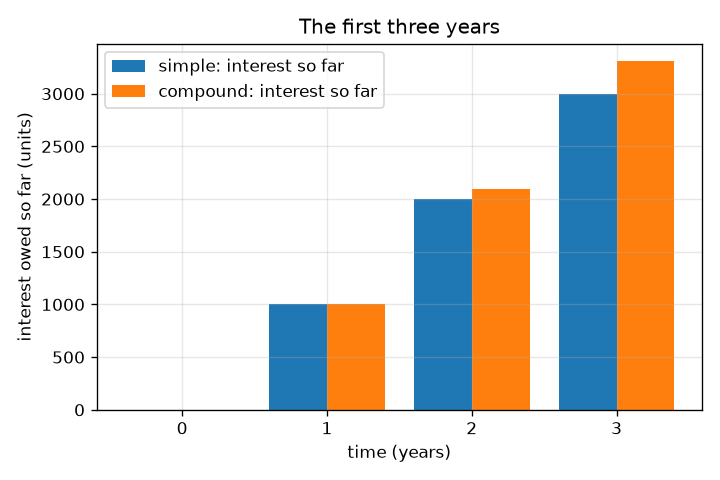
\includegraphics[width=0.85\linewidth]{figures/s01_first_three_years.png}\\\small Interest owed in the first three years: equal in year 1, then compound pulls ahead.\end{center}

\subsection*{E. Worked example}
You borrow 10000 units at 10 percent a year for 3 years and repay everything at the end. How much do you owe with simple interest and with compound interest, and what is the difference?
\begin{enumerate}[nosep]
\item Simple: interest = 10000 * 0.10 * 3 = 3000, so you owe 10000 + 3000 = 13000.
\item Compound, year 1: 10000 * 1.1 = 11000.
\item Year 2: 11000 * 1.1 = 12100. Year 3: 12100 * 1.1 = 13310. (Or 10000 * 1.1\textasciicircum{}3 = 13310.)
\item Difference = 13310 - 13000 = 310 units: the interest charged on earlier interest.
\end{enumerate}
\textbf{Answer.} Simple interest: 13000 units. Compound interest: 13310 units. Compounding costs 310 more.

\subsection*{F. Questions}
\begin{enumerate}[nosep]
\item \textbf{Conceptual.} Why does compound interest grow faster than simple interest, even though both use the same rate? When are they equal?
\item \textbf{Numerical.} You borrow 5000 units at 8 percent a year for 2 years. Find the amount owed with simple and with compound interest. Check that your answers are sensible.
\item \textbf{Graph and simulation interpretation.} In the graph for 10000 units at 10 percent, what are the amounts owed after 20 years, and what does the widening gap between the curves tell you?
\item \textbf{Design and optimisation challenge.} Design: a friend offers 10000 units for 5 years at 12 percent simple interest. A bank offers the same loan at 10 percent compound. Which is cheaper over 5 years? Would your answer change at 20 years?
\end{enumerate}

\section{Session 2: Compound growth and the EMI}

\subsection*{A. Real-world problem}
Most loans are paid back in equal monthly instalments, the EMI (equated monthly instalment). Where does that number come from? How much of each payment is interest? Why does stretching a loan to make the EMI smaller cost so much more in the end? And of two offers with different rates and fees, which one is cheaper? General education with made-up offers; not financial advice.

\subsection*{B. Concept and theory}
If interest is added n times a year, A = P (1 + r/n)\textasciicircum{}(n t). Raising n makes A grow, but only up to the limit P e\textasciicircum{}(r t) (continuous compounding). For a loan repaid in n months at the same instalment E, with monthly rate i = annual rate / 12, the balance after each month is balance x (1 + i) - E. Choosing E so that the balance reaches exactly zero after n months gives EMI = P i (1+i)\textasciicircum{}n / ((1+i)\textasciicircum{}n - 1). Month k's interest part is balance x i and its principal part is E minus that. Total interest = n E - P. The effective annual rate (1 + i)\textasciicircum{}12 - 1 is what the monthly compounding really costs over a year.

\begin{itemize}[nosep]
\item P: principal: the amount borrowed (units)
\item i: monthly rate = annual rate / 12 (per month)
\item n: number of monthly payments (tenure) (months)
\item E: EMI: the equal monthly payment (units per month)
\item A: amount after compounding (units)
\item r, t: annual rate (fraction) and time in years for compound growth (per year, years)
\end{itemize}

\begin{equation*}
A=P\left(1+\frac{r}{n}\right)^{nt}\ \longrightarrow\ P\,e^{rt}\quad (n\to\infty)
\end{equation*}

\begin{equation*}
E=\frac{P\,i\,(1+i)^{n}}{(1+i)^{n}-1},\qquad i=\frac{\text{annual rate}}{12}
\end{equation*}

\begin{equation*}
B_{k}=B_{k-1}(1+i)-E,\qquad B_0=P,\ B_n=0
\end{equation*}

\begin{equation*}
\text{interest}_k=B_{k-1}\,i,\qquad \text{principal}_k=E-\text{interest}_k,\qquad \text{total interest}=nE-P
\end{equation*}

\begin{equation*}
\text{effective annual rate}=(1+i)^{12}-1
\end{equation*}

\begin{center}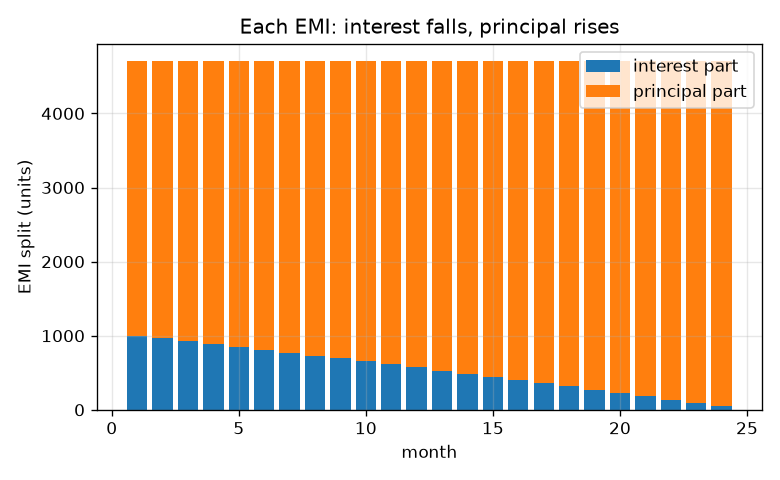
\includegraphics[width=0.85\linewidth]{figures/s02_amortisation.png}\\\small Each EMI split into interest and principal over 24 months.\end{center}

\subsection*{E. Worked example}
Borrow 100000 units at 12 percent a year for 24 months. Find the EMI, the interest and principal of month 1, and the total interest, then check the EMI by simulating the balance.
\begin{enumerate}[nosep]
\item Monthly rate i = 12 / 12 percent = 0.01 and n = 24. (1.01)\textasciicircum{}24 = 1.2697.
\item EMI = 100000 * 0.01 * 1.2697 / (1.2697 - 1) = 1269.7 / 0.2697 = 4707.35 units.
\item Month 1: interest = 100000 * 0.01 = 1000.00; principal = 4707.35 - 1000.00 = 3707.35.
\item Total interest = 24 * 4707.35 - 100000 = 12976.33 units.
\item Check by simulation: start at 100000; each month multiply by 1.01 and subtract 4707.35. After 24 months the balance is 0 (to rounding).
\end{enumerate}
\textbf{Answer.} EMI 4707.35 units per month; month 1 has 1000.00 interest and 3707.35 principal; total interest 12976.33 units; the simulated balance reaches zero after 24 payments.

\subsection*{F. Questions}
\begin{enumerate}[nosep]
\item \textbf{Conceptual.} Why is the interest part of the EMI large at the start and small at the end, although the EMI itself never changes?
\item \textbf{Numerical.} Find the EMI and the total interest for 100000 units at 12 percent a year over 12 months. State the units and do a sanity check.
\item \textbf{Graph and simulation interpretation.} In the tenure graph for 100000 units at 12 percent, what happens to the EMI and to the total interest when the tenure grows from 12 to 60 months?
\item \textbf{Design and optimisation challenge.} Design: you can afford an EMI of at most 4000 on a 100000 loan at 12 percent and want the least total interest. Which tenure in the table (12, 24, 36, 48 or 60 months) do you pick? Separately, compare Offer A (9.0 percent a year with a 2 percent fee, 36 months) and Offer B (9.8 percent, no fee, 36 months) for 100000. Which is cheaper in total?
\end{enumerate}

\section{Session 3: Simulating real loans: prepayment, rate changes and flat rates}

\subsection*{A. Real-world problem}
Real loans are messier than the formula. You may pay extra when you have spare money, the bank may change the rate, an offer of 'flat 8 percent' may sound cheaper than it is, and money loses value with inflation. A simulator can answer all of these. General education with made-up numbers; not financial advice.

\subsection*{B. Concept and theory}
The simulator repeats one step per month: add interest (balance x annual rate / 12), subtract the payment, and subtract any lump sum. It reproduces the EMI formula exactly when nothing else changes, which validates it. A prepayment reduces the balance at once, so every later month's interest is smaller and the loan ends earlier. If the rate changes, either the tenure changes (keep the EMI) or the EMI is recomputed for the remaining months. A flat-rate offer charges rate x P x years of interest on the original amount and splits P plus interest into equal instalments; since you repay principal every month, the true rate is the one for which the reducing-balance EMI equals the flat instalment, found by bisection or Newton's method. Payments in the future are worth less today: the present value of a payment E in month k is E / (1 + inflation/12)\textasciicircum{}k. Failure cases: an EMI above the share of income you can spare, and a payment below the monthly interest, which makes the balance grow (negative amortisation).

\begin{itemize}[nosep]
\item B\_k: balance after month k (units)
\item i: monthly rate = annual rate / 12 (per month)
\item E: payment each month (units per month)
\item L: lump sum paid after month m (units)
\item flat: flat annual rate quoted on the original P (per year)
\item x: unknown true annual rate to be found (per year)
\item infl: yearly inflation (per year)
\end{itemize}

\begin{equation*}
B_k=B_{k-1}(1+i)-E-L\,[k=m]
\end{equation*}

\begin{equation*}
E_{\text{flat}}=\frac{P\,(1+\text{flat}\cdot n/12)}{n}
\end{equation*}

\begin{equation*}
f(x)=\text{EMI}(P,x,n)-E_{\text{flat}}=0,\qquad x_{j+1}=x_j-\frac{f(x_j)}{f'(x_j)}
\end{equation*}

\begin{equation*}
PV=\sum_{k=1}^{n}\frac{E}{(1+\text{infl}/12)^{k}}
\end{equation*}

\begin{equation*}
P_{\max}=E_{\max}\,\frac{(1+i)^{n}-1}{i\,(1+i)^{n}},\qquad E_{\max}=\text{income}\times\text{share}
\end{equation*}

\begin{center}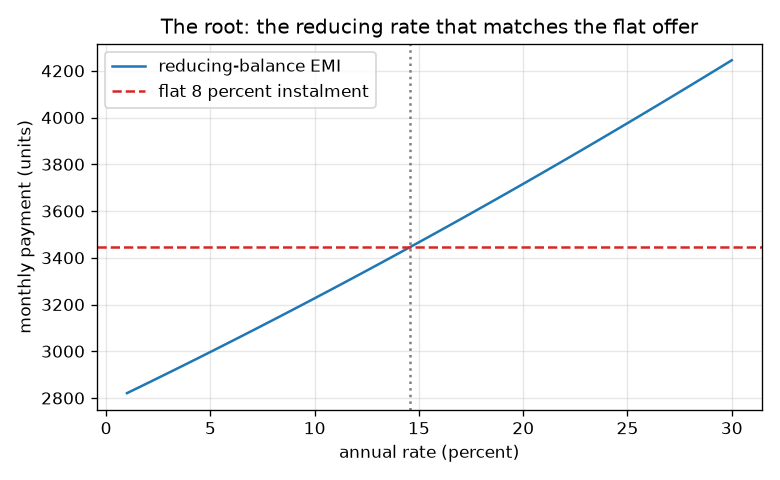
\includegraphics[width=0.85\linewidth]{figures/s03_flat_vs_reducing.png}\\\small Reducing-balance payment against rate; the flat 8 percent instalment meets it near 14.5 percent.\end{center}

\subsection*{E. Worked example}
A loan of 200000 units at 12 percent a year over 60 months has an EMI of 4448.89. You pay a lump sum of 50000 after month 12 and keep paying the same EMI. When does the loan end and how much interest is saved? Then find the true rate of a flat 8 percent, 36-month loan of 100000.
\begin{enumerate}[nosep]
\item Without prepayment the simulation ends in 60 months with total interest 66933.37.
\item With the lump sum the balance drops by 50000 at month 12; the simulation ends in 44 months with total interest 42482.30.
\item Interest saved = 66933.37 - 42482.30 = 24451.07 units; the loan ends 16 months early.
\item Flat 8 percent: interest = 100000 * 0.08 * 3 = 24000, instalment = 124000 / 36 = 3444.44.
\item Solve EMI(100000, x, 36) = 3444.44 for x by bisection: x = 14.548 percent a year. A reducing 8 percent loan has EMI 3133.64 and interest 12810.92, just over half of the flat interest.
\end{enumerate}
\textbf{Answer.} The loan ends in 44 months and saves 24451.07 units of interest. 'Flat 8 percent' is really about 14.548 percent a year on the reducing balance.

\subsection*{F. Questions}
\begin{enumerate}[nosep]
\item \textbf{Conceptual.} Why does a lump sum paid early save more interest than the same lump sum paid late?
\item \textbf{Numerical.} A flat 8 percent loan of 100000 units for 3 years: find the total interest and the instalment, and compare the interest with a reducing 8 percent loan. Is the flat loan really cheaper than its name suggests?
\item \textbf{Graph and simulation interpretation.} In the balance graph, what happens at the month of the lump sum, and how does the later part of the curve differ from the plain loan?
\item \textbf{Design and optimisation challenge.} Design: monthly income is 30000 units and you decide an EMI may use at most 40 percent. At 12 percent over 60 months, what is the largest loan you can take? Then explain what goes wrong if someone pays only 800 per month on a 100000 loan at 12 percent.
\end{enumerate}

\section{Real-world mini-project}
\textbf{Compare three made-up loan offers.} You need 300000 units for 60 months. Offer X: 10.5 percent reducing balance with a 1 percent fee. Offer Y: 9.5 percent reducing balance with a 3 percent fee. Offer Z: 'flat 6 percent', no fee. All are made up. For each offer find the EMI or instalment, the total cost (interest plus fee), the effective annual rate when the fee is taken out of the money you receive, and the interest saved by a 50000 lump sum after month 12 (assume Z allows no benefit). Use \texttt{simulate}, \texttt{emi}, \texttt{flat\_instalment} and \texttt{true\_annual\_rate\_bisect} from Session 3. General education only, not advice.

\section{The path ahead}
\begin{enumerate}[nosep]
\item \textbf{Session 4: All-in cost with extra charges.} A function returning the effective annual rate of a loan with a percentage fee and a fixed insurance amount, both deducted from the money received.
\item \textbf{Session 5: Step-up EMI.} A solver for the first-year EMI when the payment rises 5 percent every 12 months and the balance must end at zero.
\item \textbf{Session 6: Prepayment penalty optimiser.} A search over lump-sum months with a 2 percent penalty on the lump sum.
\item \textbf{Session 7: Rate path engine.} A simulator that takes a list of rates and recomputes the EMI every 6 months.
\item \textbf{Session 8: Reproduce the Target.} A 48-frame animation with three linked panels, saved as a GIF under 3 MB.
\end{enumerate}

\section{Answers and hints}

\subsection*{Session 1}
\begin{enumerate}[nosep]
\item \textbf{Conceptual.} Hint: Ask what the interest is charged on in the second year. Solution: With simple interest the interest is always charged on the original principal. With compound interest last year's interest has been added to the debt, so this year's interest is charged on a larger amount: interest on interest. They are equal after exactly one year (and at time zero); from year 2 onwards compound is larger.
\item \textbf{Numerical.} Hint: Simple: 5000 (1 + 0.08 * 2). Compound: 5000 * 1.08 * 1.08. Solution: Simple: 5000 * 1.16 = 5800 units. Compound: 5000 * 1.1664 = 5832 units. Sanity check: both exceed 5000, compound is slightly larger than simple, and the difference (32 units) is 5000 * 0.08\textasciicircum{}2, the interest on the first year's interest.
\item \textbf{Graph and simulation interpretation.} Hint: Read the two curves at 20 years on the horizontal axis. Solution: Simple interest gives 30000 units, compound gives about 67275 units. The gap keeps widening because simple interest adds the same slice each year while compound interest adds a slice that grows with the debt. Long debts are where compounding matters most.
\item \textbf{Design and optimisation challenge.} Hint: Compute both amounts for 5 years, then think about which curve bends upwards. Solution: Friend: 10000 * (1 + 0.12 * 5) = 16000 units. Bank: 10000 * 1.1\textasciicircum{}5 = 16105.10 units. Over 5 years the friend's offer is cheaper, by about 105 units, although its rate is higher. Assumption: nothing is repaid before the end and no fees. Over much longer times the compound curve bends upwards and eventually passes any straight line, so the answer can reverse. The lesson: compare the total amount over the time you will really borrow, not the headline rate.
\end{enumerate}

\subsection*{Session 2}
\begin{enumerate}[nosep]
\item \textbf{Conceptual.} Hint: What is the interest in a month charged on? Solution: Interest each month is charged on the balance still owed. Early on the balance is large, so the interest part is large and little of the EMI is left to reduce the balance. Each payment lowers the balance, so the next interest part is smaller and more of the fixed EMI goes to principal. In the example the interest part falls from 1000.00 to 46.61 while the principal part rises from 3707.35 to 4660.74.
\item \textbf{Numerical.} Hint: Use i = 0.01 and n = 12 in the EMI formula; total interest = n E - P. Solution: EMI = 8884.88 units per month. Total interest = 12 * 8884.88 - 100000, which is about 6618.55 units. Sanity check: the average balance is about half of 100000, so interest is about 12 percent of 50000 = 6000, close to the exact 6618.55.
\item \textbf{Graph and simulation interpretation.} Hint: Compare the table values at 12 and at 60 months. Solution: The EMI falls from 8884.88 to 2224.44 units, about a quarter of the size, but the total interest rises from 6618.55 to 33466.69 units, more than five times as much. A longer tenure lowers the monthly burden but you pay interest on the balance for much longer.
\item \textbf{Design and optimisation challenge.} Hint: Check the EMI at each tenure first. For the offers, total cost = n E - P + fee. Solution: At 24 months the EMI is 4707.35, above 4000, so it fails; 36 months has EMI 3321.43 and total interest 19571.52, the shortest tenure that fits and so the least interest. Offers: A has EMI 3179.97 and total cost 16479.04 (interest plus fee); B has EMI 3217.34 and total cost 15824.13. B is cheaper in total even though its rate is higher and its EMI larger, because A's fee outweighs its lower rate over this tenure. Assumptions: the fee is paid in cash up front, no prepayment, rates fixed.
\end{enumerate}

\subsection*{Session 3}
\begin{enumerate}[nosep]
\item \textbf{Conceptual.} Hint: Think about how many months of interest the removed balance would otherwise have been charged. Solution: A lump sum cuts the balance from that month on, so every later month's interest is smaller. Paid early, it affects many more months of interest than paid late. For a 50000 lump sum in the 200000 example, paying after month 1 saves 32313.54 units, more than the 24451.07 saved by paying after month 12.
\item \textbf{Numerical.} Hint: Flat interest = P x rate x years. Reducing EMI uses the Session 2 formula. Solution: Flat: interest 24000, instalment 3444.44. Reducing 8 percent: EMI 3133.64, interest 12810.92. The flat loan costs nearly twice the interest; its true rate is about 14.5 percent. The word 'flat' hides that you repay principal each month but are still charged on the full amount.
\item \textbf{Graph and simulation interpretation.} Hint: Look for a sudden drop and compare the slopes afterwards. Solution: At the lump-sum month the balance drops suddenly by the lump sum (the kink). After it the curve is lower and reaches zero earlier, at month 44 instead of month 60, because less interest is added each month and so more of each EMI goes to principal.
\item \textbf{Design and optimisation challenge.} Hint: Maximum EMI = 12000. Invert the EMI formula. For the second part compare 800 with the monthly interest. Solution: Maximum EMI = 0.40 * 30000 = 12000. The largest loan is about 539460.46 units (check: its EMI is 12000). In the second case the monthly interest is 100000 * 0.12 / 12 = 1000, more than the 800 paid, so the balance grows: after 60 months it is 116333.93 and the loan never clears (negative amortisation). Trade-off: a larger loan or a longer tenure lowers the payment but increases risk and total interest. This is a simplified classroom model, not advice.
\end{enumerate}

\section{How to join}
Read \texttt{CONTRIBUTING.md} in the repository, then pick an issue labelled \texttt{good first issue}. Repository: \url{https://github.com/KrunalPanchal1995/openloan}

\end{document}
